\section{Gestión de Incidentes}\label{sec:gestionDeIncidentes}

El objetivo de la gestión de incidentes es identificar y registrar de manera temprana los defectos y mejoras en el producto, 
con el fin de corregirlos oportunamente. Para ello, el equipo decidió utilizar Azure DevOps para reportar los incidentes. Se detalló una 
descripción de cada incidente, las causas conocidas, el tipo (defecto o mejora), quién lo reportó, la fecha y el lugar donde fue detectado.

Los incidentes serán registrados en Azure Boards, donde se registrarán, priorizarán y gestionarán todos los problemas detectados 
durante las fases de prueba. El flujo de trabajo para cada incidente será el siguiente:

\begin{enumerate}
    \item \textbf{Registro del Incidente}\\
    El tester será responsable de registrar el incidente en Azure Boards, proporcionando una descripción detallada que incluya:
    \begin{itemize}
        \item Título breve y conciso.
        \item Severidad asignada.
        \item Pasos para reproducir el problema.
        \item Datos específicos utilizados para la prueba (si corresponde).
        \item Capturas de pantalla, registros o cualquier otro dato relevante que facilite la resolución.
    \end{itemize}
    \item \textbf{Asignación de Prioridad}\\
    El Product Owner (PO) revisará cada incidente registrado y asignará una prioridad basada en el impacto que tiene en el sistema y en los objetivos del sprint. 
    Esto asegura que los problemas más críticos se aborden primero.
    \item \textbf{Análisis y Diagnóstico}\\
    El equipo de desarrollo, junto con los revisores de código, analizará los incidentes para identificar la causa del incidente. Durante esta etapa, se puede convocar 
    a sesiones de revisión conjunta para comprender mejor el problema, discutir posibles soluciones y estimar el tiempo de corrección.
    \item \textbf{Implementación de la Solución}\\
    Una vez identificado el problema, el desarrollador asignado trabajará en la corrección. Se asegurará de:
    \begin{itemize}
        \item Realizar los cambios necesarios en el código.
        \item Ejecutar pruebas unitarias y funcionales para verificar que la solución resuelve el problema sin introducir nuevos defectos.
        \item Notificar al equipo de QA cuando la corrección esté lista para ser validada.
    \end{itemize}
    \item \textbf{Validación y Cierre}\\
    El equipo de QA ejecutará pruebas de validación para asegurar que el incidente ha sido resuelto y que no afecta otras funcionalidades. Si la solución es efectiva,
    el incidente se marcará como resuelto y se cerrará. Si persisten problemas, se reabre el incidente para un análisis adicional.
    \item \textbf{Reporte de Progreso y Estado}\\
    Periódicamente, se generarán un informe de seguimiento utilizando la siguiente plantilla que resumirá:
    \begin{itemize}
        \item Número total de incidentes reportados.
        \item Número de incidentes abiertos, en proceso y cerrados.
        \item Severidad de los incidentes pendientes.
        \item Estos informes permitirán al equipo tener una visión clara del estado del sistema y del progreso en la resolución de problemas, ayudando a tomar decisiones 
        informadas sobre la planificación de futuras iteraciones.
    \end{itemize}
    \item \textbf{Reuniones de Seguimiento}\\
    Durante las reuniones de seguimiento de sprint (retrospectivas), se revisará el estado de los incidentes y se discutirán bloqueadores o problemas recurrentes que
    necesiten atención especial. Este espacio también servirá para ajustar prioridades si se identifican nuevos riesgos o problemas críticos.
    \item \textbf{Gestión de Incidentes Recurrentes}\\
    En caso de que un mismo tipo de problema reaparezca en múltiples ocasiones, se convocará a una sesión de análisis profundo para entender las causas subyacentes.
    Para esta etapa el equipo dispone de las herramientas Pareto Ponderado y 5 Por qués.
\end{enumerate}


La gestión de los incidentes se representa a través del flujo indicado en la figura \ref{fig:flujoIncidentes}.

\begin{figure}[H]
    \centering
    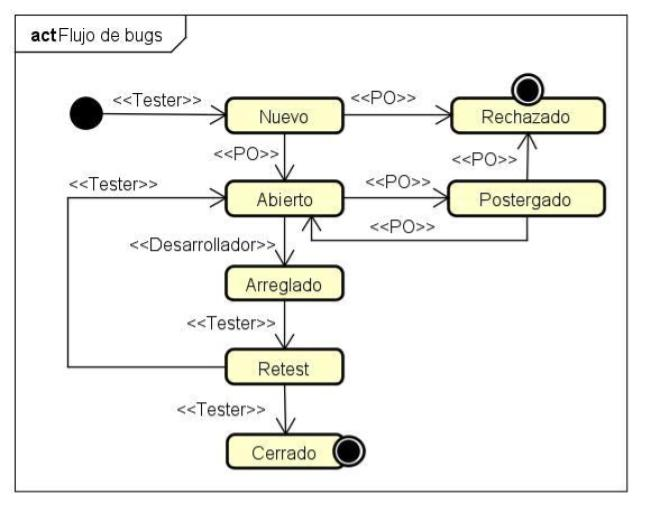
\includegraphics[width=0.8\textwidth]{../imagenes/secciones/8-Gestion-de-la-Calidad/Flujo gestion de incidentes.jpg}
    \caption{Flujo de Gestión de Incidentes}
    \label{fig:flujoIncidentes}
\end{figure}

La tabla \ref{tab:estadosIncidentes} describe los posibles estados de un incidente y su significado.

\begin{table}[H]
    \centering
    \begin{tabular}{p{3cm} p{10cm}}
    \hline
    \textbf{Estado} & \textbf{Descripción} \\ \hline
    Nuevo & El incidente ha sido registrado en Azure Boards y está pendiente de revisión por el Product Owner. \\ \hline
    Rechazado & El Product Owner ha revisado el incidente y ha determinado que no es válido o no es necesario corregirlo. \\ \hline
    Postergado & El incidente ha sido validado pero no se ha asignado a un sprint específico. \\ \hline
    Abierto & El incidente ha sido validado y asignado a un sprint específico para su corrección. \\ \hline
    Arreglado & El desarrollador ha implementado una solución y está pendiente de validación por el equipo de QA. \\ \hline
    Restest & El incidente ha sido validado por el equipo de QA y se ha detectado que la solución no es efectiva. \\ \hline
    Cerrado & El incidente ha sido validado por el equipo de QA y se ha confirmado que la solución es efectiva. \\ \hline
    \end{tabular}
    \caption{Estados de un Incidente}
    \label{tab:estadosIncidentes}
\end{table}

\subsection{Severidad de un incidente}
La severidad se clasifica en 5 niveles descritos en la tabla \ref{tab:severidadIncidentes}.

\begin{table}[H]
    \centering
    \begin{tabular}{p{3cm}p{10cm}}
    \hline
    \textbf{Severidad} & \textbf{Significado} \\ \hline
    Bloqueante & Implica que una funcionalidad no se pueda utilizar y no exista otra forma de realizar esa misma acción. El sistema falla por completo o una funcionalidad esencial no está disponible. \\ \hline
    Crítica & Implica que una funcionalidad no se puede utilizar pero existe una alternativa para completar la acción. \\ \hline
    Alta & Defecto en una funcionalidad prioritaria del sistema o que tiene impacto secundario en una funcionalidad prioritaria del mismo. Una funcionalidad importante está afectada, pero el sistema aún es utilizable con limitaciones. \\ \hline
    Medio & Cualquier defecto que impacte en una funcionalidad secundaria. Problemas en funcionalidades no críticas que afectan parcialmente al usuario. \\ \hline
    Bajo & Cualquier defecto ortográfico o de visualización. Problemas menores. \\ \hline
    \end{tabular}
    \caption{Severidad y detalles posibles de un Incidente}
    \label{tab:severidadIncidentes}
\end{table}

\subsection{Priorización de Incidentes}

La priorización de los incidentes será de acuerdo a la clasificación de severidad y la tabla de prioridades \ref{tab:prioridadIncidentes}.


\begin{table}[H]
    \centering
    \begin{tabular}{p{3cm}p{10cm}}
    \hline
    \textbf{Prioridad} & \textbf{Significado} \\ \hline
    Alta & Debe resolverse de inmediato para que el desarrollo o las pruebas continúen sin interrupciones significativas. \\ \hline
    Media & Se puede resolver en la siguiente iteración o versión, pero sigue siendo importante. \\ \hline
    Baja & Puede resolverse cuando haya tiempo disponible o en futuras versiones, no es urgente. \\ \hline
    Sugerencias & Mejoras o recomendaciones que no son urgentes ni críticas para el funcionamiento actual. \\ \hline
    \end{tabular}
    \caption{Prioridad de un Incidente}
    \label{tab:prioridadIncidentes}
\end{table}


% Análisis de Causa Raíz (Root Cause Analysis)
% Utilización de técnicas como los 5 Porqués para identificar y abordar las causas subyacentes de los problemas encontrados durante el desarrollo y las pruebas​​. Esta técnica será implementada utilizando la siguiente plantilla.

% Pareto ponderado - Impacto de los errores en el código (bugs)
% Frente a la posibilidad de que existan diversas fuentes de errores que puedan impactar negativamente la calidad del producto desarrollado se entiende necesario disponer de una herramienta de priorización de las causas para atacar las más importantes y no todas al mismo tiempo. 
% Si bien existe más de una técnica que nos permita lograr el objetivo, un diagrama de pareto ponderado es la más sencilla de implementar. Además, es de una potencia estadística contundente ya que aproximadamente el 20% de los orígenes de problemas reportarán el 80% de los errores introducidos en el producto.
% El análisis se llevará a cabo utilizando la siguiente plantilla.